\documentclass[11pt]{article}
\usepackage{fullpage}
\usepackage{graphicx}
\title{Interaction Design: Usability Measure}
\author{Miguel Vazquez}
\begin{document}
\maketitle
\section{Experiment}
For this experiment three different operating systems were used with each of the individual tasks. The three tasks were finding a file titled “Find ME”, connecting to Wi-Fi, and finally finding and starting the calculator. Each test subject was timed, their reactions, satisfaction, and proficiency with each operating system was recorded. The three measured metrics were Learnability. Efficiency and Satisfaction.
\section{Usability Metrics}

\subsection{Learnability}
Although most of the test subjects have had prior experience with Mac and Windows Linux proved to be a learning experience for everyone. Where everyone knew about using search to find what they need they were unaware of how to do it with Linux. It did have a magnifying glass image which instantly called to them. However once they clicked on it they did not realize that the an appropriate folder to search from was needed. They were used to Windows and Mac which will search the entire computer and this caused for them to have to learn about choosing it correctly. They also had to learn that calculator is not a document so it will not be found with the search they were used to and had to click on the tab that seemed to be somewhat hidden and overlooked by people.

\subsection{Efficiency}
As was stated everyone had proficiency with Mac and Windows. This meant everyone used the search for each operating system. This caused them to find the file with ease and did not need to go through different folders to find the file. For the second task which was setting Wi-Fi everyone recognizes a symbol for Wi-Fi which although different with each operating system remains relatively the same. The test subjects were drawn to the symbol once told the task which is why the lowest times were with this task. As for the final efficiency slowed once the search was of no use in Linux. Without this tool the subjects were handicapped and found it difficult to adapt or try something new. This of course led to some time spent trying to force search to work and then giving up and searching for a solution. It should be noted however that for the Mac most users knew of the Launchpad and did the simple gesture to get the calculator widget which is what caused the fast calculator times with the Mac.

\subsection{Satisfaction}
Most subjects were satisfied with Mac and Windows. The only complaint related to Windows was that its search was rather slow. Linux however was seen with much hostility. Some subjects commented that Linux is “stupid”, “idiotic” and even a “waste of time.” As stated users had difficulty accomplishing the tasks on Linux which of course led to their dissatisfaction. They had just done the same tasks twice and with relative ease and now found themselves struggling what they had just done easily a couple of minutes ago. This of course led to their dissatisfaction towards Linux.

\section{Examination Of Data}
The data collected from these experiments is shown below.

\begin{figure}[h!]
  \centering
    \includegraphics[width= 1\textwidth]{./Images/Data_table}
  \caption{Data collected}
\end{figure}

\begin{figure}[h!]
  \centering
    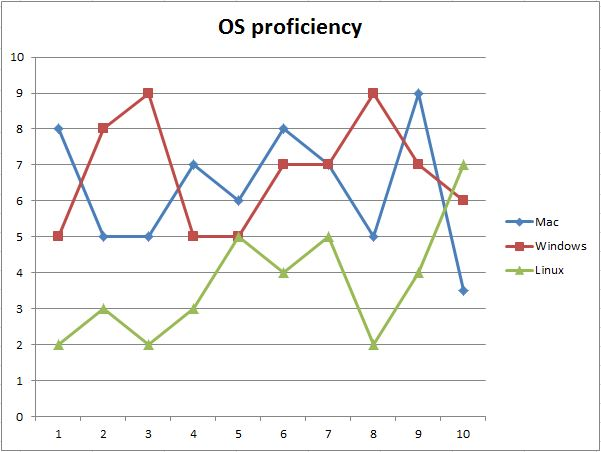
\includegraphics[width=0.75\textwidth]{./Images/Proficiency}
  \caption{Proficiency Values}
\end{figure}

\begin{figure}[h!]
  \centering
    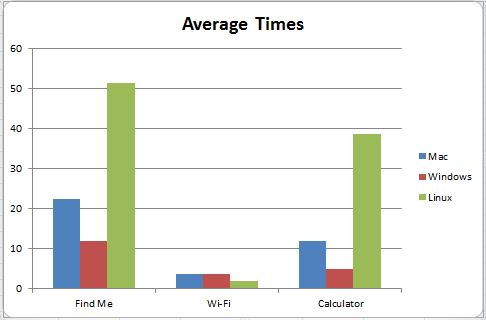
\includegraphics[width=0.75\textwidth]{./Images/Average_Times}
  \caption{Average Time Values}
\end{figure}

\begin{figure}[h!]
  \centering
    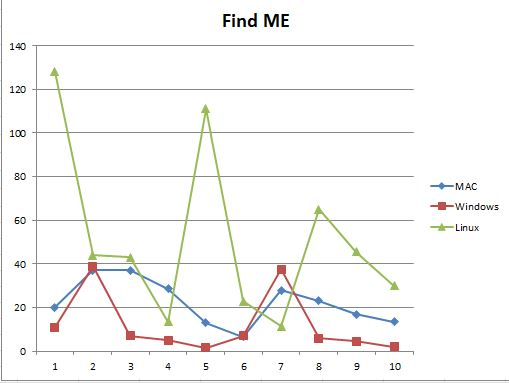
\includegraphics[width=0.75\textwidth]{./Images/Find_ME}
  \caption{Find Me search times}
\end{figure}

\begin{figure}[h!]
  \centering
    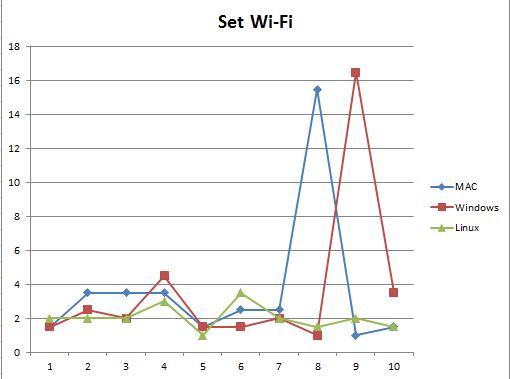
\includegraphics[width=0.75\textwidth]{./Images/Wi-Fi}
  \caption{Wi-Fi set-up times}
\end{figure}

\begin{figure}[h!]
  \centering
    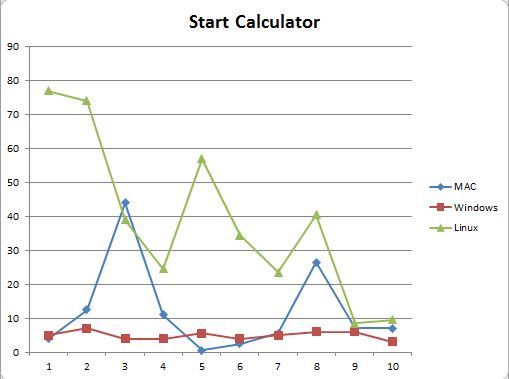
\includegraphics[width=0.75\textwidth]{./Images/Calculator}
  \caption{Calculator times}
\end{figure}

\end{document}